%!TEX root = ../../prace.tex

\section{Stavební akce}

\textbf{Destruktor} umožňuje mazat bloky. Po jeho výběru je vidět červený outline vybraného bloku.

\begin{figure}[!ht]\centering
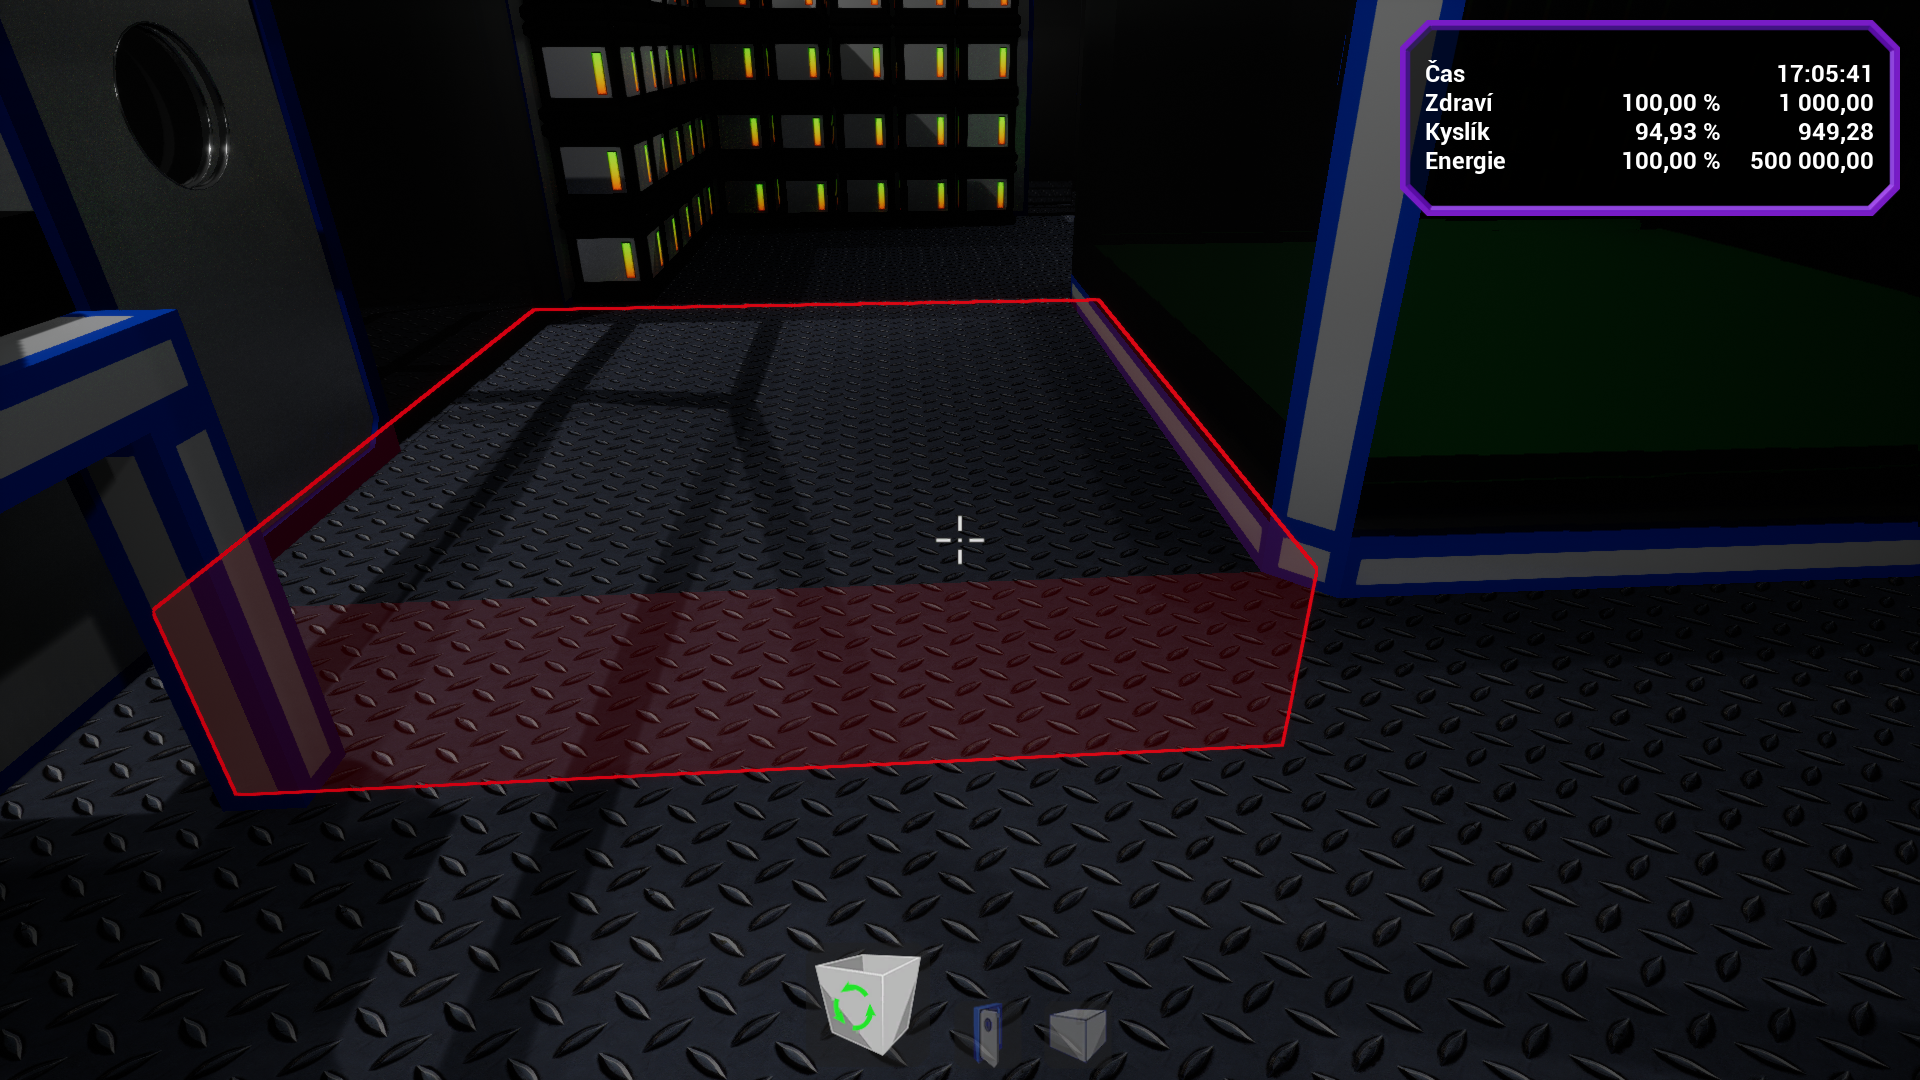
\includegraphics[ width=140mm]{../img/user/buildActions/delete}

\caption{Stavění - smazat}
\label{fig:user_buildActions_delete}

\end{figure}

\FloatBarrier

Pokud vybereme umístění nového bloku, vidíme žlutě hranice sousedního bloku, ke kterému blok přistavujeme. Stavěný / umisťovaný blok musí mít dostatečné místo pro svoje umístění. Dále je potřeba mít s~sebou dostatečně velkou zásobu energie (dle energetické náročnosti bloku).

\begin{figure}[!ht]\centering
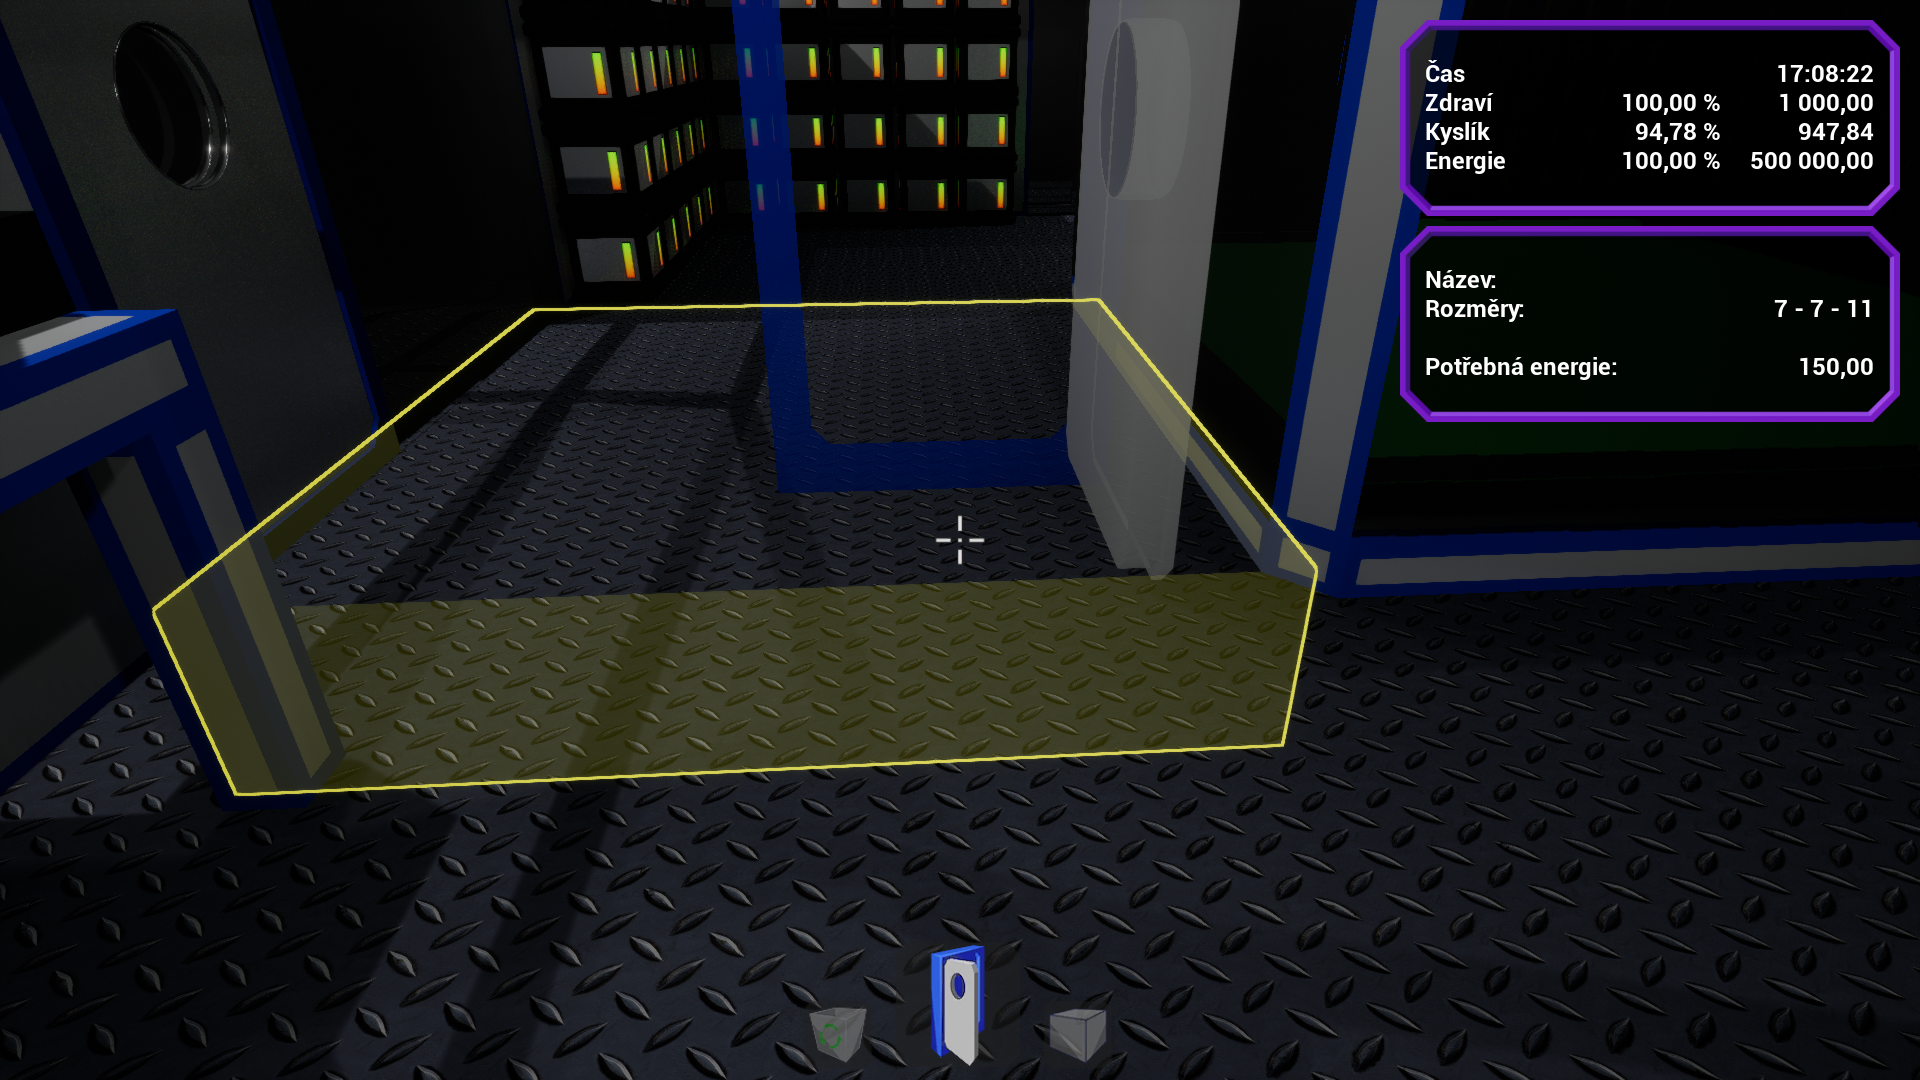
\includegraphics[ width=140mm]{../img/user/buildActions/place}

\caption{Stavění - umístit}
\label{fig:user_buildActions_place}

\end{figure}

\FloatBarrier

Blok je též možný rotovat (Klávesy v~sekci Insert .. Page Down, případně jejich ekvivalenty 7,8,9,4,5,6).

\begin{figure}[!ht]\centering
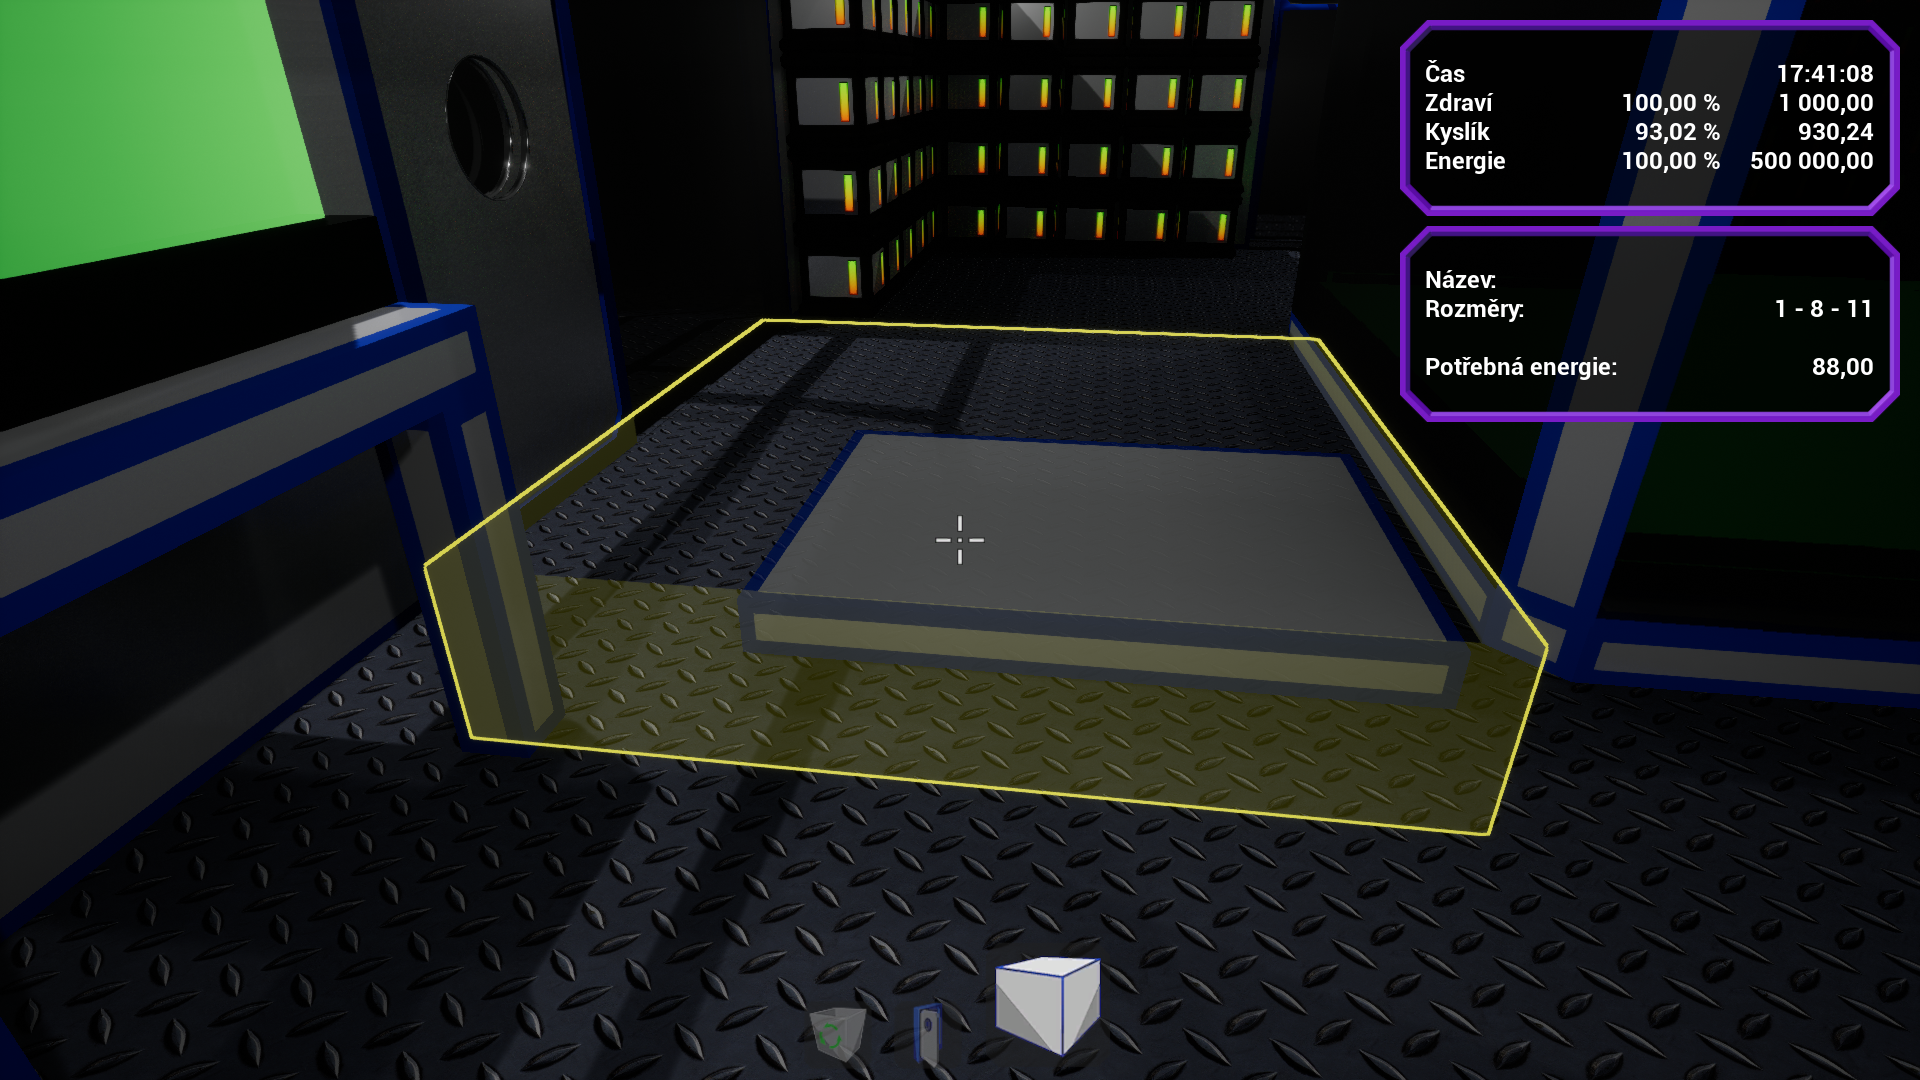
\includegraphics[ width=140mm]{../img/user/buildActions/place_Rotate}

\caption{Stavění - rotace}
\label{fig:user_buildActions_place_Rotate}

\end{figure}

\FloatBarrier

Pokud bylo umístění v~pořádku, blok již není nadále průhledný a~hráči ubyla energie. Pokud je zapnut kreativní mód, energie samozřejmě neubývá.

\begin{figure}[!ht]\centering
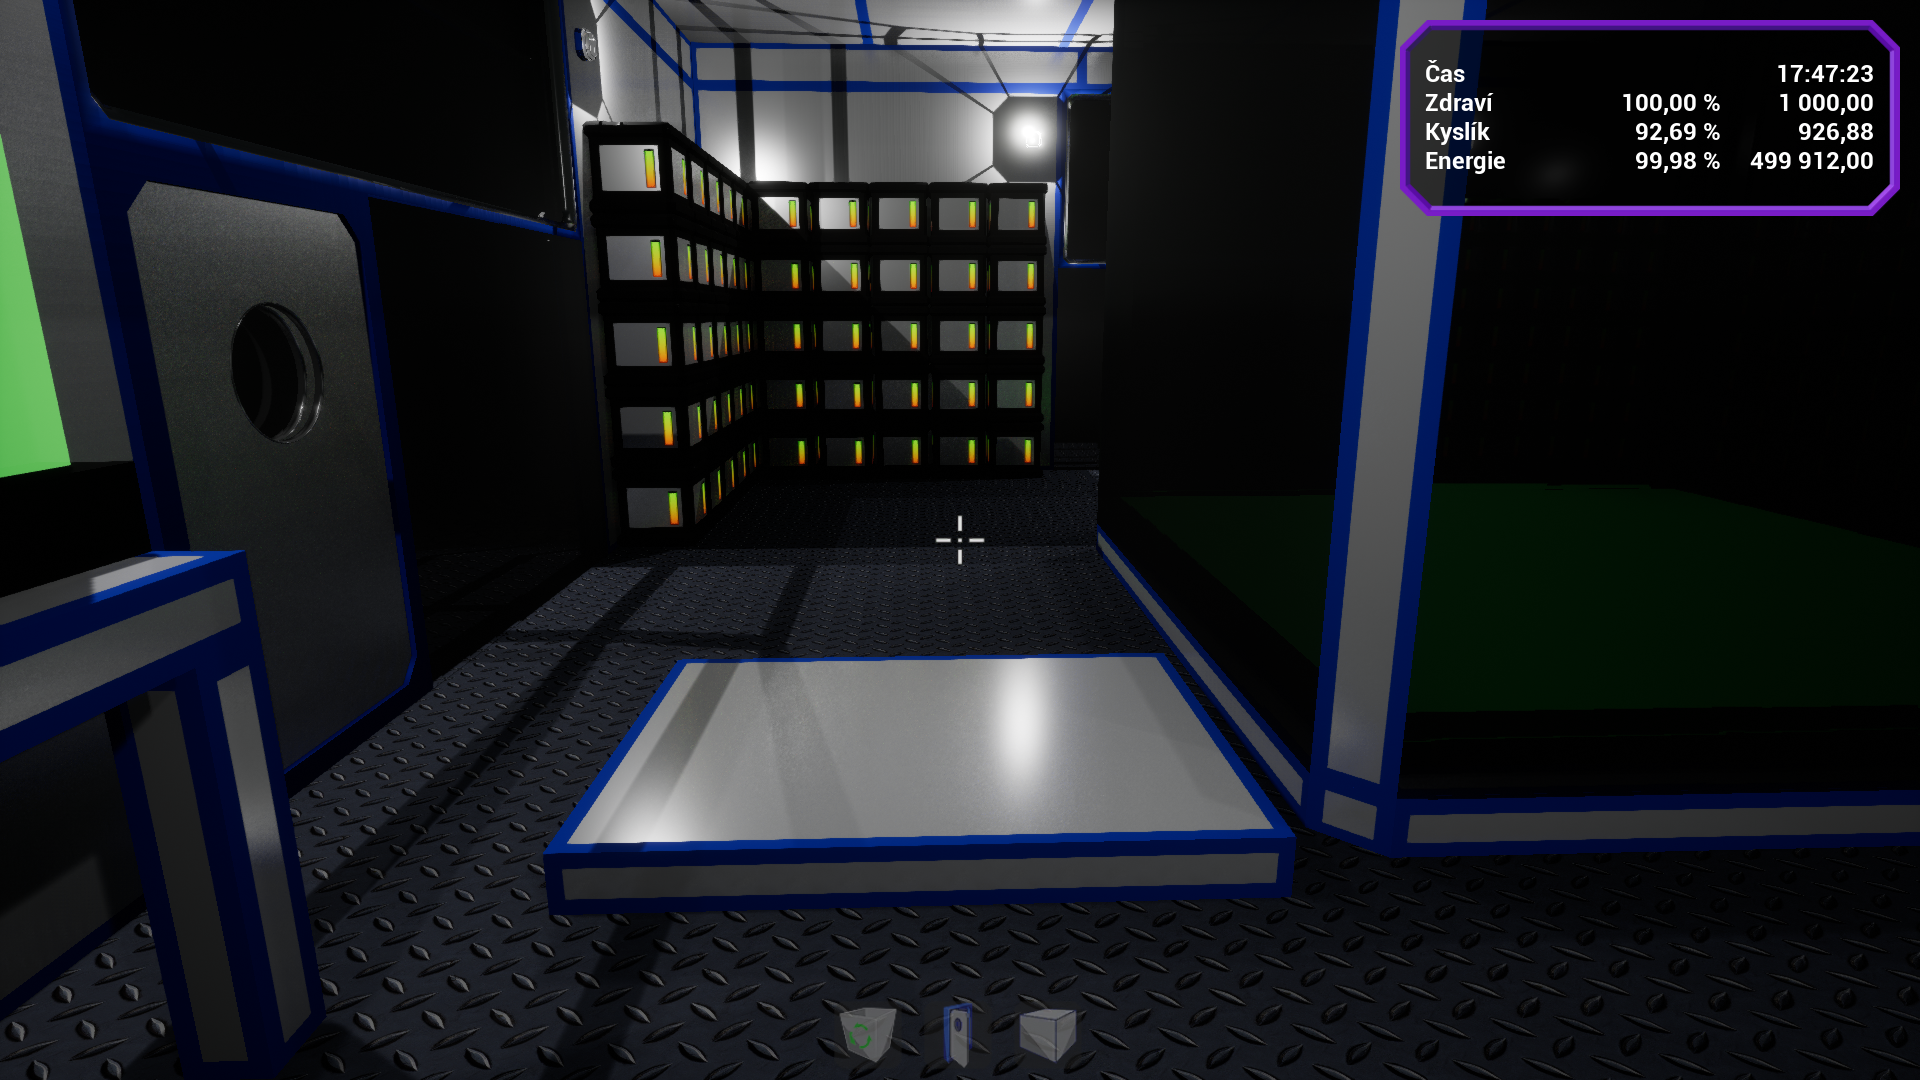
\includegraphics[ width=140mm]{../img/user/buildActions/placeAfter}

\caption{Stavění - po umístění}
\label{fig:user_buildActions_placeAfter}

\end{figure}


\FloatBarrier